% amdg
% use t hese as templates:
% https://aaai.org/ocs/index.php/AAAI/AAAI18/paper/view/16970/16653
% https://aaai.org/ocs/index.php/AAAI/AAAI18/paper/view/16932/16630
% https://aaai.org/ocs/index.php/AAAI/AAAI18/paper/view/17022/16605 

\def\year{2020}\relax
%File: formatting-instruction.tex
\documentclass[letterpaper]{article} % DO NOT CHANGE THIS
\usepackage{aaai20}  % DO NOT CHANGE THIS
\usepackage{times}  % DO NOT CHANGE THIS
\usepackage{helvet} % DO NOT CHANGE THIS
\usepackage{courier}  % DO NOT CHANGE THIS
\usepackage[hyphens]{url}  % DO NOT CHANGE THIS
\usepackage{graphicx} % DO NOT CHANGE THIS
\urlstyle{rm} % DO NOT CHANGE THIS
\def\UrlFont{\rm}  % DO NOT CHANGE THIS
\usepackage{graphicx}  % DO NOT CHANGE THIS
\frenchspacing  % DO NOT CHANGE THIS
\setlength{\pdfpagewidth}{8.5in}  % DO NOT CHANGE THIS
\setlength{\pdfpageheight}{11in}  % DO NOT CHANGE THIS
%\nocopyright
%PDF Info Is REQUIRED.
% For /Author, add all authors within the parentheses, separated by commas. No accents or commands.
% For /Title, add Title in Mixed Case. No accents or commands. Retain the parentheses.
\pdfinfo{
	/Title (Dynamic Curriculum Learning with Item Response Theory)
	/Author (John P. Lalor, Hong Yu)
} %Leave this
\pdfinfo{
	/Title (Dynamic Curriculum Learning with Item Response Theory)
	/Author (Anonymous AAAI Submission)
} %Leave this

	
% /Title ()
% Put your actual complete title (no codes, scripts, shortcuts, or LaTeX commands) within the parentheses in mixed case
% Leave the space between \Title and the beginning parenthesis alone
% /Author ()
% Put your actual complete list of authors (no codes, scripts, shortcuts, or LaTeX commands) within the parentheses in mixed case. 
% Each author should be only by a comma. If the name contains accents, remove them. If there are any LaTeX commands, 
% remove them. 

% DISALLOWED PACKAGES
% \usepackage{authblk} -- This package is specifically forbidden
% \usepackage{balance} -- This package is specifically forbidden
% \usepackage{caption} -- This package is specifically forbidden
% \usepackage{color (if used in text)
% \usepackage{CJK} -- This package is specifically forbidden
% \usepackage{float} -- This package is specifically forbidden
% \usepackage{flushend} -- This package is specifically forbidden
% \usepackage{fontenc} -- This package is specifically forbidden
% \usepackage{fullpage} -- This package is specifically forbidden
% \usepackage{geometry} -- This package is specifically forbidden
% \usepackage{grffile} -- This package is specifically forbidden
% \usepackage{hyperref} -- This package is specifically forbidden
% \usepackage{navigator} -- This package is specifically forbidden
% (or any other package that embeds links such as navigator or hyperref)
% \indentfirst} -- This package is specifically forbidden
% \layout} -- This package is specifically forbidden
% \multicol} -- This package is specifically forbidden
% \nameref} -- This package is specifically forbidden
% \natbib} -- This package is specifically forbidden -- use the following workaround:
% \usepackage{savetrees} -- This package is specifically forbidden
% \usepackage{setspace} -- This package is specifically forbidden
% \usepackage{stfloats} -- This package is specifically forbidden
% \usepackage{tabu} -- This package is specifically forbidden
% \usepackage{titlesec} -- This package is specifically forbidden
% \usepackage{tocbibind} -- This package is specifically forbidden
% \usepackage{ulem} -- This package is specifically forbidden
% \usepackage{wrapfig} -- This package is specifically forbidden
% DISALLOWED COMMANDS
% \nocopyright -- Your paper will not be published if you use this command
% \addtolength -- This command may not be used
% \balance -- This command may not be used
% \baselinestretch -- Your paper will not be published if you use this command
% \clearpage -- No page breaks of any kind may be used for the final version of your paper
% \columnsep -- This command may not be used
% \newpage -- No page breaks of any kind may be used for the final version of your paper
% \pagebreak -- No page breaks of any kind may be used for the final version of your paperr
% \pagestyle -- This command may not be used
% \tiny -- This is not an acceptable font size.
% \vspace{- -- No negative value may be used in proximity of a caption, figure, table, section, subsection, subsubsection, or reference
% \vskip{- -- No negative value may be used to alter spacing above or below a caption, figure, table, section, subsection, subsubsection, or reference

\usepackage{algorithm}
\usepackage{algpseudocode}
\usepackage{amsmath}
\usepackage{booktabs}
\usepackage{microtype}
\usepackage{subcaption}

\setcounter{secnumdepth}{2} %May be changed to 1 or 2 if section numbers are desired.

% The file aaai20.sty is the style file for AAAI Press 
% proceedings, working notes, and technical reports.
%
\setlength\titlebox{2.5in} % If your paper contains an overfull \vbox too high warning at the beginning of the document, use this
% command to correct it. You may not alter the value below 2.5 in
\title{Dynamic Curriculum Learning with Item Response Theory}
%Your title must be in mixed case, not sentence case. 
% That means all verbs (including short verbs like be, is, using,and go), 
% nouns, adverbs, adjectives should be capitalized, including both words in hyphenated terms, while
% articles, conjunctions, and prepositions are lower case unless they
% directly follow a colon or long dash
\author{
	John P. Lalor \\
	University of Notre Dame \\
	john.lalor@nd.edu
	\And 
	Hong Yu \\
	University of Massachusetts \\
	hong.yu@uml.edu
}

\author{
	Anonymous AAAI 2020 Submission
}

\begin{document}
\maketitle 
\begin{abstract}
	Curriculum learning (CL) is a popular and well-studied method for machine learning model training.
	However, most CL methods make assumptions (both implicit and explicit) about the easiness or difficulty of training examples when building curricula for learning.
	In this work we show that modeling difficulty using psychometric methods is more effective than baseline training and CL with heuristic measures of difficulty such as sentence length.
	We introduce a dynamic curriculum learning strategy that probes model competency at each training epoch to select the best training examples at that point in time.
	The dynamic model adds data at a rate commensurate with the model's capability, instead of restricting data due to an unnecessarily restrictive heuristic.
	Analysis demonstrates that these methods are more efficient than existing CL methods and capture instances of easy items that are overlooked by existing heuristics (e.g. long sentences that are easy).
%CL has been shown to be effective.
%Many measures of ``difficulty'' are based on heuristics and not on true difficulty.
%we want to change that by leveraging methods from psychometrics.
%Experiments on vision and language data show that using learned difficulty and ability to set up a curriculum is effective.
%Curriculum that is dynamically determined by the current competency of the model as estimated by Item Response Theory. 
\end{abstract}

\section{Introduction}
- go over CL
- why it works
- why there are currently issues with it (heuristics)
- bottlenecks to some of the existing approaches

Curriculum learning is a well-studied area of machine learning.
Prior work has shown that building a curriculum of training data where easy examples are shown first can speed up learning and improve generalization, a result that has also been shown in humans \cite{bengio_curriculum_2009,platanios_competence-based_2019} (also cite hadi). 
The basic premise is that machine learning (ML) models are trained according to a ``curriculum'' that sorts training examples according to difficulty.
At first, the model is trained with only the easiest examples, and more difficult examples are gradually added according to some schedule.
A major gain for CL methods is that model convergence can often be quicker when the model is trained according to some curriculum \cite{bengio_curriculum_2009,platanios_competence-based_2019}.
Model efficiency has always been a major aim of the research community (\textbf{cite old papers}), but recently with the size of models continuing to grow and better understanding of the impact of model training on the environment there is a renewed need for efficiency \cite{strubell_energy_2019}.

A major drawback of existing CL techniques is that they rely on heuristics to measure the difficulty of data, and either ignore the competency of the model at its present state or rely on heuristics there as well.
For example, often for natural language processing (NLP) tasks, sentence length is considered a proxy for difficulty \cite{bengio_curriculum_2009,platanios_competence-based_2019}.
Similarly, the original CL paper used the number of objects in an image as a proxy for difficulty in an image recognition task \cite{bengio_curriculum_2009}.
Competency was recently introduced as a mechanism to determine when new examples should be added to the training data \cite{platanios_competence-based_2019}, however in that work the competency schedule was ad hoc, and did not actually look at the competency of the model but assumed a schedule according to learning heuristics. 
Ideally, model competency would be measured, so that the training data could be appropriately matched with the model at a given point in the training.

Recent work has shown that it is possible to estimate both the difficulty of examples and the ability of deep learning models as latent variables based on model performance using Item Response Theory (IRT) \cite{lalor_learning_2019}.
IRT is a well-studied methodology in the psychometric literature for test set construction and subject evaluation \cite{baker_item_2004}.
A typical IRT model will estimate latent parameters such as difficulty for examples under consideration for inclusion in a test set and a latent ability parameters for individuals taking the test.
This is done by administering a test to a large number of human subjects, collecting and grading their responses as correct or incorrect, and using the student-response data matrix to estimate the latent traits of the data.
Once learned, these latent parameters can be used to estimate latent ability parameters of future test-takers, based on their graded responses to the examples.
IRT has not seen wide adoption in the ML community, primarily due to the fact that fitting IRT models requires a large amount of human annotated data for each example.
However, recent work has shown that it is possible to fit IRT models using machine-generated data instead of human-generated data as the input to the IRT models \cite{lalor_learning_2019}.
Because one can learn example difficulty and subject ability together, IRT is an interesting framework to consider for the problem of CL. 

In this work we propose Dynamic Curriculum Learning with IRT (DCL-IRT), a novel framework that uses the estimated ability of a model at a specific point in the training process to identify appropriate training data.
At each training epoch, the latent ability of the model is estimated.
Based on this estimate, only training data that the model has a reasonable chance of labeling correctly is included in training.
As the model improves, the estimated ability will improve, and more training examples will be added.

Our contributions are as follows: (i) we propose a novel CL framework, DCL-IRT, which automatically selects training data based on the estimated ability of the model, (b) we show that model training using DCL-IRT leads to faster convergence than traditional training and better performance than baseline CL methods, (c) we provide an analysis of the DCL-IRT training regime to show why certain training examples hurt instead of help generalization.
This is the first work to learn a model competency during training that is directly comparable to the difficulty of the training data pool.

Code used for this work will be released upon publication, and is included as supplemental material.

\section{Methods}

In this section we first describe a typical CL framework.
We then introduce IRT for those unfamiliar with the methodology, specifically the one-parameter logistic (1PL) model, also referred to as the Rasch model \cite{rasch_studies_1960,baker_item_2004}.
Learning IRT models for machine-learning scale data sets with variational inference methods is then described, and finally we introduce the Dynamic Curriculum Learning model with IRT (DCL-IRT) for probing model ability to select training examples.

\subsection{Curriculum Learning}
\begin{figure}[ht]
	\centering 
	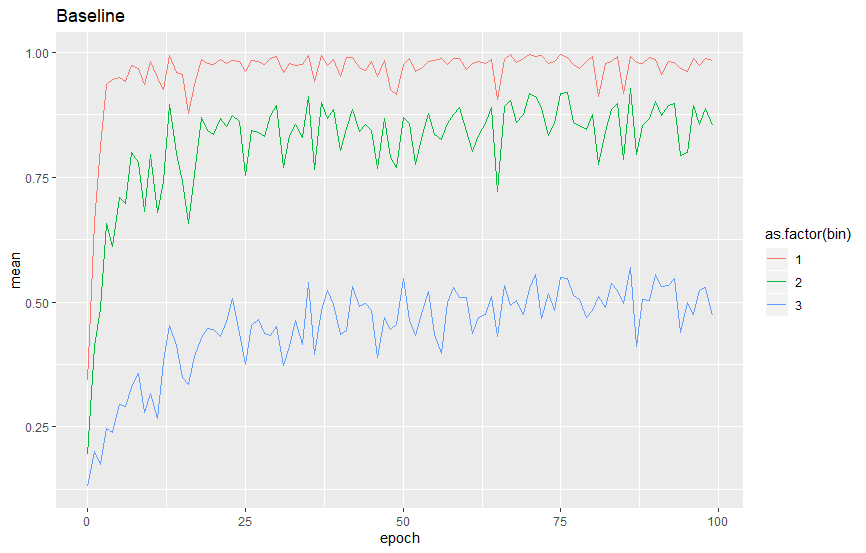
\includegraphics[width=150pt]{figs/baseline}
	\caption{A typical curriculum learning framework, where examples are added at each epoch according to (a) a learning schedule and (b) example difficulty (NEED A NEW FIG HERE)}.
	\label{fig:cl_framework} 
\end{figure}


In a traditional CL framework, training data examples are ordered according to some notion of difficulty, and the training set shown to the learner is augmented at a set pace with more and more difficult examples (Fig. \ref{fig:cl_framework}).

Typically, the model's current performance is not taken into account. 
Recent work has incorporated a notion of ``competency'' to CL \cite{platanios_competence-based_2019}.
In that work the authors structure the rate at which training examples are added based on an assumption that model competency is modeled by either a linear or root function of the training epoch.
However there are two issues with such an approach.
First, this notion of competency is artificially rigid.
If a model's competency improves quickly, more data cannot be added more quickly because the rate is predetermined.
On the other hand, if a model is slow to improve, it may struggle because more data is being added too quickly.
Second, the formulation of competency proposed by the authors reduces to a competency-free CL rate with a tuneable parameter for inclusion speed.
This heuristic notion of competency aligns with typical heuristic notions of difficulty used for CL, but in this work we do away with the heuristics and instead measure difficulty and competency directly. 

\subsection{Item Response Theory}
\label{ssec:irt} 
\subsubsection{Learning Latent Parameters with IRT}
IRT methods learn latent parameters of test set examples (called ``items'' in the IRT literature) and latent ability parameters of individual test-takers (``subjects'').
We refer to ``items'' as ``examples'' and ``subjects'' as ``models'' for clarity and consistency with the CL literature.

For a model $j$ and an example $i$, the probability that $j$ answers $i$ correctly ($z_{ij}=1$) is a function of the latent parameters of $j$ and $i$.
The one-parameter logistic (1PL) model, also known as a Rasch model, assumes a single latent difficulty parameter for examples, $b_i$ \cite{rasch_studies_1960,baker_item_2004}:
\begin{equation} 
p(z_{ij} = 1 \vert \theta_j, b_i) = \frac{1}{1 + e^{-(\theta_j - b_i)}}
\end{equation}

The probability that subject $j$ will answer item $i$ incorrectly ($z_{ij}=0$) is:
\begin{equation} 
p(z_{ij} = 0 | \theta_j, b_i) = 1 - p(y_{ij} = 1 \vert \theta_j, b_i)
\end{equation} 

With a 1PL model, there is an intuitive relationship between difficulty and ability.
A model has a 50\% chance of answering an example correctly when model ability is equal to example difficulty ($\theta_j = b_i$).

More advanced IRT models that include additional latent parameters for examples such as guessing exist, but in this work we focus on the 1PL model because we are primarily interested in example difficulty.

Learning a 1PL model requires a set of $I$ examples $\{i_0, i_1, \dots, i_I\}$, a set of $J$ models $\{j_0, j_1, \dots, j_J\}$, and the binary graded responses $Z = \{\forall_{i \in I} \forall_{j \in J}: z_{ij}\}$ of the subjects to each of the items.
The likelihood of a dataset of response patterns $Z$ from multiple subjects to a set of items given the model parameters $\theta$ and $b$ is:
\begin{align} 
p(Z \vert \theta, b) &= \prod_{j=1}^J \prod_{i=1}^I p(Z_{ij}=y_{ij} \vert \theta_j, b_i)
\end{align} 
where $z_{ij} = 1$ if individual $j$ answers item $i$ correctly and $z_{ij} = 0$ if they do not.

Typically, IRT models are fit using marginal maximum likelihood (MML) estimation, where the latent ability parameters ($\theta$) are assumed to be random effects and integrated out.
Latent item parameters are estimated using an expectation maximization (EM) method \cite{bock_marginal_1981}.
These methods assume human subjects, and were typically used for relatively small data sets of no more than a hundred examples or so.


\subsubsection{IRT with VI} 
A major bottleneck of using IRT methods on machine learning data sets is the fact that each subject would have to label each (or most of) the examples in order to have enough response patterns to estimate the latent parameters.
Having humans annotate all examples in an ML data set can't be done, but recent work has shown that the human subjects can be replaced with an ensemble of machine learning models. 
The response patterns from this ``artificial crowd'' can be used to estimate item parameters by fitting IRT models using variational inference (VI) methods.
With VI, latent parameters are estimated via variational distributions \cite{natesan_bayesian_2016,lalor_learning_2019}. 

Learning the latent difficulty parameters of training examples can be done off-line using existing techniques \cite{natesan_bayesian_2016,lalor_learning_2019}.
Bayesian methods in IRT assume that the individual $\theta$ and $b$ parameters in Eq. (2) both follow Gaussian prior distributions and make inference through the resultant joint posterior distribution $\pi(\theta,b|Y)$. As this posterior is usually intractable, VI approximates it by the variational distribution:
\begin{align} 
q(\theta, b) &=  \prod_{j=1}^J \pi^\theta_j(\theta_j) \prod_{i=1}^I \pi^b_i(b_i)
\end{align} 

Where $\pi^\theta_j()$ and $\pi^b_i()$ denotes different Gaussian densities for different parameters whose means and variances are determined by minimizing the KL-Divergence between $q(\theta,b)$ and $\pi(\theta,b|Y)$.

The choice of priors in Bayesian IRT can vary.
Prior work has shown that vague and hierarchical priors are both effective \cite{natesan_bayesian_2016}.
We experiment with both in this work. A vague prior assumes $\theta_j \sim N(0, 1)$ and $b_i \sim N(0, 10^3)$, where the large variance indicates a lack of information on the difficulty parameters.
A hierarchical Bayesian model assumes
\begin{align*}
\theta_j\ |\ m_\theta, u_\theta &\sim N(m_{\theta}, u^{-1}_{\theta}) \\
b_i\ |\ m_b, u_b &\sim N(m_b, u^{-1}_b) \\
m_{\theta}, m_{b} &\sim N(0, 10^6) \\
u_{\theta}, u_b &\sim \Gamma(1, 1)
\end{align*}

We follow the results of prior work where hierarchical priors were used \cite{lalor_learning_2019}.
To learn these parameters then involves minimizing the KL divergence between $q$ and $p$: $\min KL(q \vert \vert p)$. 

% JL: if we have room, add ELBO 

\subsubsection{Scoring}
\label{ssec:scoring}
Estimating the ability of a model at a point in time is done with a ``scoring'' function. 
When example difficulties are known, model ability is estimated by maximizing the likelihood of the data given the response patterns and the example difficulties to obtain the ability estimate.
All that is required is a single forward pass of the model on the data, as is typically done with a test or validation set. 

\begin{align}
Z_j &= \forall_{y \in Y} \mathbf{I}[y_i = \hat{y_i}] \\
L(\theta_j \vert Z_j) &= p(Z_j \vert \theta_j)  \\
&= \prod_{i=1}^I p(z_{ij}=y_{ij} \vert \theta_j) 
\end{align}

% ADD MATH HERE 

\subsection{Dynamic Curriculum Learning with IRT}

We propose DCL-IRT, where training examples are selected dynamically at each training epoch based on the estimated ability of the model at that point.
With DCL-IRT, model ability can be estimated according to a well-studied psychometric framework as opposed to heuristics.
At the same time, the estimated ability of the model ($\hat{\theta}_e$) is on the same scale as the difficulty parameters of the data, so there is a principled recipe for selecting data at any given training epoch.


The first step of DCL-IRT is to estimate the ability of the model using the scoring function (\S \ref{ssec:scoring}). 
To do this we use the full training set, but crucially, only to get response data, not to update parameters. 
Model outputs are obtained for the training set, and graded as correct or incorrect as compared to the gold standard label. 
This response pattern is then used to estimate model ability at the current epoch ($\hat{\theta}_e$).

Once ability is estimated, data selection is done by comparing estimated ability to the examples' difficulty parameters.
Each example in the training pool has an estimated difficulty parameter ($b_x$).
If the difficulty of an example is less than or equal to the estimated ability, then the example is included in training for this epoch.
Examples where the difficulty is greater than estimated ability are not included.

With DCL-IRT, the training data size does not have to be monotonically increasing. If a model's performance suffers as a result of adding data too quickly, then this will be reflected in lower ability estimates, which leads to less data selected in the next epoch. 
This avoids a scenario where data is added too quickly at the expense of learning the easier examples.
At the same time, if estimated model ability is high, then more data can be added more quickly, without artificially slowing down learning.

Algorithm \ref{alg:dcl} shows all of the steps for DCL-IRT. Code implementing DCL-IRT is included as supplemental material and will be released upon publication. 

\begin{algorithm}
	\caption{Dynamic Curriculum Learning with IRT}
	\hspace*{\algorithmicindent}\textbf{Input:} (X, Y), model $\phi$, D \\
	\hspace*{\algorithmicindent}\textbf{Output:} Learned model $\phi$ 
	\begin{algorithmic}[1]
		\While{True}
			\State $\hat{Y} = \phi(X)$
			\State $\hat{\theta_e} = score(Y, \hat{Y}, D)$
			\State $X_e, Y_e = \{(x,y): d_x < \hat{\theta_e}\}$
			\State $train(\phi, X_e, Y_e)$
		\EndWhile 
		\Procedure{score}{$Y, \hat{Y}, D$}
			\State $Z = \forall_{y \in Y} \mathbf{I}[y_i = \hat{y_i}]$
			\State $\hat{\theta_e} = \operatorname*{arg\,max}_\theta p(Z \vert \theta, b)p(\theta))$
		\EndProcedure 
	\end{algorithmic} 
	\label{alg:dcl}
\end{algorithm} 

\section{Data and experiments} 

We experiment with four data sets, two from vision and two from NLP, to demonstrate the effectiveness of DCL-IRT across multiple domains: handwritten digit recognition, image recognition, sentiment analysis, and natural language inference.

\subsection{Data}
\subsubsection{MNIST}

MNIST is a popular handwritten digit recognition data set \cite{lecun_mnist_nodate}.
There are 60,000 training examples and 10,000 test examples in the data set.
We split the training set and use the first 50,000 examples for training and the last 10,000 examples as a validation set.
MNIST is a commonly used first-pass data set for machine learning experiments, but is not enough for all evaluation as performance on the data set has been above 99\% for some time.
We include MNIST as a toy example to validate our hypotheses.

\subsubsection{CIFAR} 

CIFAR is an image recognition data set across 10 classes \cite{krizhevsky_learning_2009}.
There are 50,000 training example and 10,000 test examples in the data set.
We split the training set and use the first 40,000 for training and the last 10,000 as a validation set. 

\subsubsection{SSTB} 

SSTB is an English-language sentiment analysis data set that consists of text excerpts from IMDB movie reviews with corresponding human-annotated sentiment labels \cite{socher_recursive_2013}.
There are 67,349/872/1821 examples in the SSTB training/validation/test sets respectively.

\subsubsection{SNLI} 

SNLI is an English-language natural language inference (NLI) data set that consists of human-generated sentence pairs and NLI labels (entailment, contradiction, or neutral) \cite{bowman_large_2015}.
There are 550,152/10,000/10,000 examples in the data set.

\subsection{Generating Response Patterns}

In order to learn the difficulty parameters of the data we require a data set of response patterns.
As previously mentioned, gathering enough labels for each example in the data sets to fit an IRT model would be prohibitively expensive for human annotators.
In addition, the annotation quality would be suspect due to the humans labeling tens of thousands of examples.
Therefore we used artificial crowds to generate our response patterns \cite{lalor_learning_2019}. 

Briefly, for each data set an ensemble of neural network models are trained, using different subsets of the training data set.
Training data is subsampled and corrupted (label flipping) so that performance across models in the ensemble is varied.
Each trained model then labels all of the examples (train/validation/test).
These labels are graded correct/incorrect against the gold-standard label and the output response patterns are used to fit an IRT model for the data (\S \ref{ssec:irt}).
Prior work has shown that this is an effective way to generate a set of response patterns for fitting IRT models to machine learning data \cite{lalor_learning_2019}.


\subsection{Experiments} 

In order to demonstrate the effectiveness of DCL-IRT we must show that the model is more efficient than standard supervised learning training while maintaining the level of performance in terms of test set accuracy. 
Any gains in predictive performance are an additional benefit, but are not the main goal.
With this in mind we performed the following experiment.

For each data set, we trained a standard model architecture for a set number of epochs. 
We varied the training data available to the model at each epoch based on the type of curriculum applied:

\begin{itemize}
	\item 
	Baseline: At each epoch, the model has access to all of the data, shuffled and in mini-batches
	\item 
	Ordered: At each epoch, the model has access to all of the data, but here the data is ordered according to difficulty (i.e. not shuffled) 
	\item 
	Simple-IRT: At each epoch, the model has access to $\frac{e}{N}$ training examples, where $e$ is the current epoch and $N$ is the full training set size. 
	This strategy ignores the competence of the model and only uses the example difficulty as inclusion criteria
	\item 
	DCL-IRT: At each epoch, model ability is estimated ($\hat{\theta_e}$, see \S above) and all training examples where difficulty is less that $\hat{\theta_e}$ are included.
\end{itemize}

For Ordered and Simple, there are several options available in terms of which examples are introduced first.
For each method we experiment with ordering the data in three ways:
\begin{itemize}
	\item 
	Easy-first: The data are ordered from easiest to hardest. At each epoch, more difficult examples are included in training
	\item 
	Hard-first: The data are ordered from hardest to easiest. At each epoch, easier examples are included in training
	\item 
	Middle-out: The data are ordered from smallest to largest in terms of the absolute value of the difficulty parameter. Recall that difficulty is roughly normally distributed (CLEAN THIS UP BECAUSE THAT ISN'T EXACTLY TRUE). At the first training epoch, data that are of an ``average'' difficulty are included in training. At each subsequent epoch, some data that are slightly easier and some data that are slightly harder are added to the training set.
\end{itemize}

For each data set a relatively simple model architecture was used.
Performance in terms of test set accuracy is determined by using the development set accuracy as an early stopping indicator.
Each model was trained for 200 epochs. 

- experiments: ordered vs simple vs irt, balanced vs not balanced

To compare against the current state-of-the-art for CL \cite{platanios_competence-based_2019}, we also look at the following heuristics for measuring model competency, used for introducing training data into the curriculum.
For the methods below, $t$ is the current time-step in training, $T$ is the point where the model is fully competent, $c_0$ is the initial competency. 

\begin{itemize}
	\item 
	Linear: define the proportion of training examples to include at time $t$ as $c_{linear}(t) \overset{\Delta}{=} \text{min} (1, t\frac{1-c_0}{T} + c_0)$
	\item 
	Root: $c_{sqrt}(t) \overset{\Delta}{=} \text{min}(1, \sqrt{t\frac{1-c_0^2}{T} + c_0^2})$
\end{itemize}

It is worth noting here that neither Linear nor Root actually measure competency of the model at any point. 
Instead it is assumed that the model becomes more and more competent over time.

\section{Results} 


\captionsetup[subfigure]{labelformat=empty}
\begin{figure*}[th!]
	\centering
	\begin{subfigure}[b]{0.45\textwidth}
		\centering
		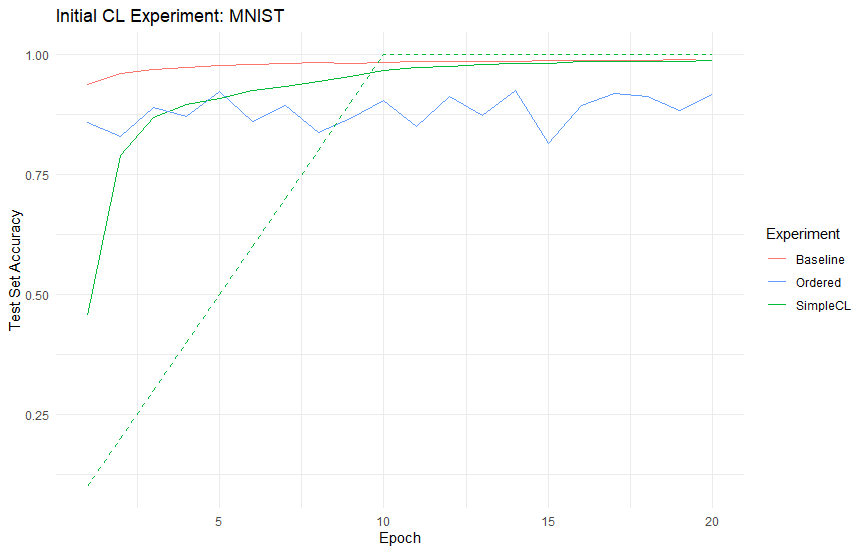
\includegraphics[width=0.9\columnwidth]{figs/cl_mnist}
		\caption{\label{fig:cl_mnist}} 
		\vspace{-2em} 
	\end{subfigure} 
	\begin{subfigure}[b]{0.45\textwidth}
		\centering
		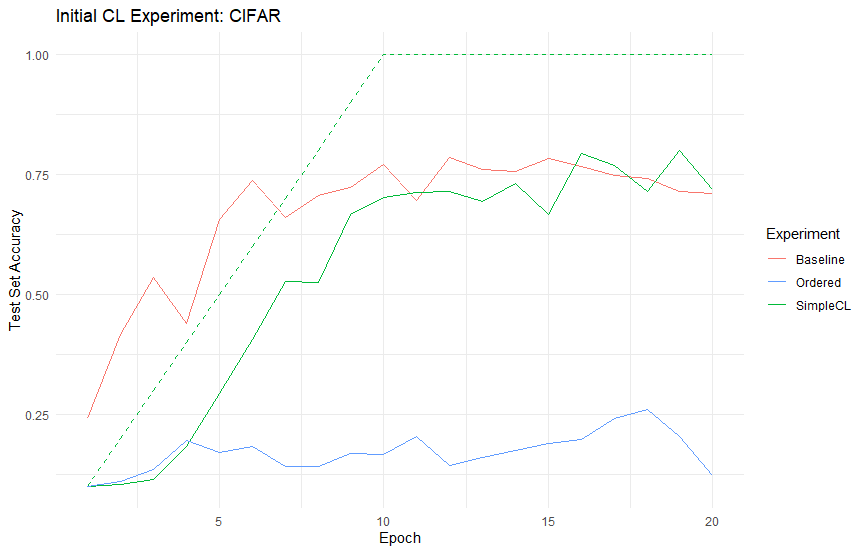
\includegraphics[width=0.9\columnwidth]{figs/cl_cifar}
		\caption{\label{fig:cl_cifar}} 
		\vspace{-2em} 
	\end{subfigure} 
	
	\caption{Test set accuracy as a function of training epoch.}
	\label{fig:acc_viz}
\end{figure*}

\captionsetup[subfigure]{labelformat=empty}
\begin{figure*}[th!]
	\centering
	\begin{subfigure}[b]{0.45\textwidth}
		\centering
		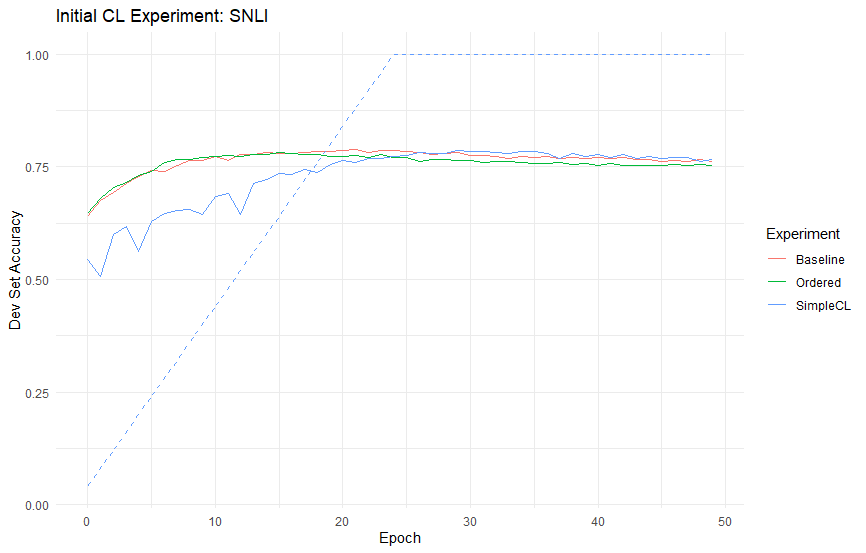
\includegraphics[width=0.9\columnwidth]{figs/cl_snli}
		\caption{\label{fig:cl_snli}} 
		\vspace{-2em} 
	\end{subfigure} 
	\begin{subfigure}[b]{0.45\textwidth}
		\centering
		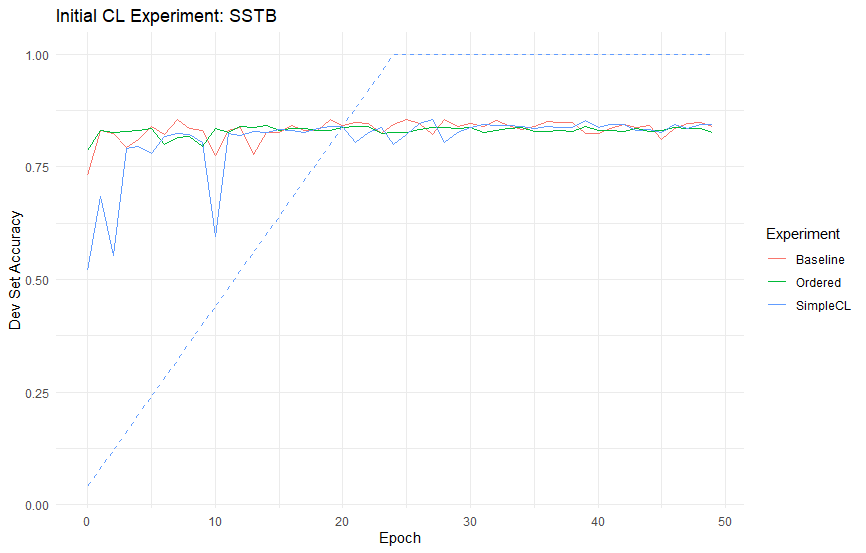
\includegraphics[width=0.9\columnwidth]{figs/cl_sstb}
		\caption{\label{fig:cl_sstb}} 
		\vspace{-2em} 
	\end{subfigure} 
	
	\caption{Test set accuracy as a function of training epoch.}
	\label{fig:acc_nlp}
\end{figure*}

- plots and tables 

- really show that using our method is efficient and practical 

Using IRT leads to quicker convergence for the trained models (Figure XX).
The vertical lines in each plot indicate the point at which the model has converged, based on early stopping using the development set accuracy.
In most cases DCL-IRT leads to the fastest convergence, however for XX using the Simple-IRT curriculum ordered easiest to hardest leads to the fastest convergence.
In all cases some use of IRT to determine the curriculum improves over the baseline training criterion. 

By using DCL-IRT a curriculum can adapt during training according to the estimated ability of the model.
DCL-IRT adds or removes training data based not on a fixed step schedule but rather by probing the model at each epoch and using the estimated ability to match data to the model (Figure XX).
This way if a model has a high estimated ability early in training, then more data can be added to the training set more quickly, and learning isn't artificially slowed down due to the curriculum schedule.
For each data set in question, DCL-IRT adds training data more quickly than a more traditional CL schedule, which leads to faster convergence.

Performance for ordered is strange.
Sometimes it works very well (SSTB), sometimes it doesn't work at all (SNLI).
More work is required here to see what is going on (PUT IT IN THE ANALYSIS SECTION).

Even though training with these curriculum use less data than the baseline, efficiency does not have a significant negative impact on generalizability in terms of test set performance (Table \ref{tab:costs}).
The number of training examples required to reach convergence is lower than the baseline in each case for DCL-IRT.
Change in performance compared to the baseline is often lower, but the delta is extremely small (usually XX or YY relative change). 
In particular, the amount of data needed to achieve very high performance on the SSTB task is roughly 25\% of what a typical training regiment would require.


\begin{table*}[h!]
	\centering 
	\begin{tabular}{cccccc}
		\toprule
		Data Set & Experiment & Training Examples & $\Delta_b$ (\%) & Accuracy (\%) & $\Delta_b$ (\%)\\ 
		\midrule
		MNIST & Baseline & 10,320,000& 100.0&	99.26&	0
		 \\
		 \cmidrule{2-6}
		& EasyFirst & 7,620,000&	73.84&	99.17&	-0.09
		 \\
		& MiddleOut & 6,420,000	&\bf 62.21	&99.2&	-0.06
		 \\
		& Ordered &10,020,000&	97.09&	97.06&	-2.22
		 \\
		& Theta& 8,986,612&	87.08&	99.23&	\bf -0.03
		 \\
		\midrule
		CIFAR & Baseline &  6,750,000& 	100.0&	86.61&	0
		 \\
		 \cmidrule{2-6}
		& EasyFirst & 6,900,000&	102.22&	85.54	&\bf -1.24
		 \\
		& MiddleOut & 3,250,000&	\bf 48.15&	85.54&	\bf -1.24
		 \\
		& Ordered &7,250,000&	107.41&	39.04	&-54.92
		 \\
		& Theta &3,671,016	&54.39&	83.32&	-3.80
		 \\
		\midrule
		SSTB & Baseline &  8,687,892 	&100.0	&85.71&	0
		\\
		\cmidrule{2-6}
		& EasyFirst & 2,912,757	&\bf 33.53&	85.38&	-0.39
		 \\
		& MiddleOut & 8,553,148	&98.45&	85.66&	-0.06
		 \\
		& Ordered & 2,155,136&	24.81&	86.92&	\bf 1.41
		 \\
		& Theta &2,993,225&	34.45&	85.32&	-0.46
		 \\
		\midrule
		SNLI & Baseline &  10,983,680& 	100.0&	78.08&	0
		 \\
		 \cmidrule{2-6}
		& EasyFirst & 25,839,060&	235.25&	77.64& \bf	-0.56
		 \\
		& MiddleOut &29,655,888&	270.00&	75.31&	-3.55
		 \\
		& Ordered & 98,853,120&	900.00&	11.86&	-84.81
		 \\
		& Theta& 14,118,510&	\bf 128.54&	77.34&	-0.95
		 \\
		\bottomrule 
	\end{tabular}
	\label{tab:costs}
\end{table*}


\begin{table*}[h!]
	\centering 
	\begin{tabular}{cccc}
		\toprule
		Data Set & Experiment & Mean & Variance \\ 
		\midrule
		MNIST & Baseline & 99.24&	0.0003
		\\
		\cmidrule{2-4}
		& EasyFirst & 99.17&	0.0004
		\\
		& MiddleOut & 99.13&	0.0005
		\\
		& Theta& 99.23&	 0.0003
		\\
		\midrule
		CIFAR & Baseline & 85.85 &	0.412
		\\
		\cmidrule{2-4}
		& EasyFirst & 85.53	&0.181
		\\
		& MiddleOut & 85.31&0.301
		\\
		& Theta &83.84& 0.278
		\\
		\midrule
		SSTB & Baseline &  &	0
		\\
		\cmidrule{2-4}
		& EasyFirst & &	-0.39
		\\
		& MiddleOut & &	-0.06
		\\
		& Ordered & &	 1.41
		\\
		& Theta &&	-0.46
		\\
		\midrule
		SNLI & Baseline & &	0
		\\
		\cmidrule{2-4}
		& EasyFirst & & 	-0.56
		\\
		& MiddleOut &&	-3.55
		\\
		& Ordered & &	-84.81
		\\
		& Theta& &	-0.95
		\\
		\bottomrule 
	\end{tabular}
	\label{tab:robustness}
\end{table*}



\subsection{Performance by Difficulty}
Does using DCL-IRT for training lead to a more interpretable output in terms of test set performance?
That is, when a curriculum is employed, does the model perform better on easier test examples than difficult ones?
A comparison of methods on test data binned by difficulty shows that model performance is similar when test set difficulty is taken into account (Figure XX).
The main difference is that for the baseline models, performance is stratified by difficulty almost immediately, and there are small improvements across groups during training, while for the CL methods, there is consistent improvement across groups as training continues, and more data is added. 


\section{Related work}

Lots to do here. need a thorough lit review as part of this paper 

Since it's original proposal, CL has become a well-studied area of machine learning (CITE BENGIO).
The primary focus has been on new methods to identify easy and difficult examples in order to build a curriculum. 
Originally, CL methods were evaluated on toy data sets with heuristic measures of difficulty.
For example, on a shapes data set, shapes with more sides were considered more difficult than shapes with fewer sides.
Similarly, sentences with more words were considered more difficult than sentences with fewer words.

Further work on CL has looked at estimating example difficulty by querying the model being trained (CITE EXAMPLES).
Model confidence, example entropy, and other metrics (LIST) have been considered as proxies for difficulty.
However, these all assume that a model uncertainty is equivalent to difficulty.
It is often the case, particularly in deep learning, that a model will overestimate confidence for examples due to the fact that the model is incentivized to push output probabilities to 1 for training examples (CITE ZOUBIN's work here).
These output probabilities are not aligned with a notion of difficulty, and may negatively impact the estimation of such.
What's more, most work relies on a rigid schedule that does not take into account the competency of the model at a point in the training process.

Recent work has shown that spaced repetition strategies can be effective for improving model performance (CITE HADI).
Instead of using a traditional CL setup, spaced repetition bins examples based on estimated difficulty.
The bins are shown to the model at differing intervals so that more difficult examples are seen more frequently than easier examples.
This method has been shown to be effective for human learning, and results demonstrate effectiveness on NLP tasks as well.

Recent work has shown that measuring model competence during training to determine which examples to include at a training epoch further improves performance by matching data to model competency \cite{platanios_competence-based_2019}.
However, in that work the model of competency is based on a heuristic rate of knowledge acquisition, and does not actually measure model competency.
To the best of our knowledge this is the first work to match model ability at a point in training with appropriate training data in a curriculum learning framework.


\section{Conclusion} 

DCL-IRT is the first curriculum learning method to dynamically probe a model during training to estimate model ability at a point in time.
Knowing the model's ability allows for data to be selected for training that is appropriate for the model and is not rigidly tied to a heuristic schedule.
Learning with IRT CL strategies leads to more efficient models.
%Although performance is slightly lower, the gains in efficiency more than balance the trade-off.
The difference in performance is small for many tasks, but being able to cut training data in half (or less) allows for the use of certain models in many more cases, and also allows for more researchers to work on problems where huge computing and storage resources may not be available.

Even though it is dynamic, DCL-IRT employs a simple curriculum schedule: only include examples where difficulty is less than estimated ability.
However, being able to estimate ability on the fly with IRT opens up as a research area the following: what is the best way to build a curriculum, knowing example difficulty and model ability?
It may be the case that only data with difficulty within a range of ability (higher and lower) is better, and the training set shifts as the model improves.
There are many directions to take this, and this will be an exciting area of work moving forward.

\bibliographystyle{aaai}
\bibliography{library}


\end{document}